\newchap{Linguistic Background}
\label{chap:ling-background}

This chapter sets out the linguistic background needed in order to get a better understanding of how spoken and written language relate. It covers the basics of phonetics and phonology, writing systems and the relatively new field of corpus phonetics. After setting this foundation I will have a look at the relation of spoken and written language. 


\section{Phonemes and syllables}
\label{phonology}
Given that phonetics and phonology is a sub-area of traditional linguistics and often only touched on superficially in computational linguistics, I will summarise the most important assumptions and terms concerning said field. A very important terminological distinction is between phonetics and phonology. While phonetics refers to the study of actual sounds, phonology refers to the study of sound \textit{systems}. In phonetics, it is not so much important what the different sounds mean, but how they are produced and perceived and what different sounds a human being can produce and perceive at all. When it comes to human communication using spoken language, many of these sounds are not actually used to produce distinguishable meaning. This is why on the other hand phonology is important to describe the set of distinguishable sounds that make up a language. For example: the letter /r/ in English can be pronounced in many different ways in a specific word like `request'. I can roll the /r/ like it is common in Spanish or I can pronounce it like an /r/ in German. None of those pronunciations produces a change in meaning. Others might say I have an accent or I speak a dialect but usually people will understand. This means that there exist many different \textit{phonetic} sounds but only one \textit{phonological} or \textit{phonemic}. Those sounds are referred to as phone and phoneme respectively. While there are infinitely many phones, there are only finitely many phonemes in a language. Also, in one language there is typically a set of phones that is used by the majority of speakers of this language that can replace phonemes and does not change the meaning. Sounds that can replace another sound without changing the original meaning are referred to as `allophones'. Each language has therefore a set of phonemes, a phoneme inventory, and a set of allophones. How phonemes and allophones are used depends a lot on the dialect and idiosyncratic language use.  

Not all different possible sounds are actually considered qualitatively `good' sounds of a language. Usually there is a subset of all possible phones that is accepted as `good quality sounds' within all different dialects of a language \citep{Intro.2007}. An obvious example being loudness: Although very silent speech produces correct phones, these are not `good quality' as they simply cannot be understood. Or speaking in English with hardly any mouth and tongue movement. Although this produces understandable sound, it is not generally considered good speech. 

It is important to note at this point that the terms phonetic and phonemic respectively phone and phoneme are sometimes used interchangeably. Their linguistic definition as given above is clear while the definition on the computational side is often less strict. Strictly speaking phonemic transcriptions are not allowed to contain allophones but should write the respective phoneme. This will not always be the case when it comes to data used in language technology \citep{Lee&Ashby.2020}. 


%\begin{figure}[t!]
%{\large
%\vowelvunit=4em
%\vowelhunit=4em
%\begin{center}
%\begin{vowel}
%	\putvowel{\small{front}}{0\vowelhunit}{-0.3\vowelvunit}
%	\putvowel{\small{central}}{2\vowelhunit}{-0.3\vowelvunit}
%	\putvowel{\small{back}}{4\vowelhunit}{-0.3\vowelvunit}
%	\putvowel{\small{close}}{-1\vowelhunit}{0\vowelvunit}
%	\putvowel{\small{close-mid}}{-0.33\vowelhunit}{1\vowelvunit}
%	\putvowel{\small{open-mid}}{0.33\vowelhunit}{2\vowelvunit}
%	\putvowel{\small{open}}{1\vowelhunit}{3\vowelvunit}
%	\putcvowel[l]{i}{1}
%	\putcvowel[r]{y}{1}
%	\putcvowel[l]{e}{2}
%	\putcvowel[r]{\o}{2}
%	\putcvowel[l]{\textepsilon}{3}
%	\putcvowel[r]{\oe}{3}
%	\putcvowel[l]{a}{4}
%	\putcvowel[r]{\textscoelig}{4}
%	\putcvowel[l]{\textscripta}{5}
%	\putcvowel[r]{\textturnscripta}{5}
%	\putcvowel[l]{\textturnv}{6}
%	\putcvowel[r]{\textopeno}{6}
%	\putcvowel[l]{\textramshorns}{7}
%	\putcvowel[r]{o}{7}
%	\putcvowel[l]{\textturnm}{8}
%	\putcvowel[r]{u}{8}
%	\putcvowel[l]{\textbari}{9}
%	\putcvowel[r]{\textbaru}{9}
%	\putcvowel[l]{\textreve}{10}
%	\putcvowel[r]{\textbaro}{10}
%	\putcvowel{\textschwa}{11}
%	\putcvowel[l]{\textrevepsilon}{12}
%	\putcvowel[r]{\textcloserevepsilon}{12}
%	\putcvowel{\textsci\ \textscy}{13}
%	\putcvowel{\textupsilon}{14}
%	\putcvowel{\textturna}{15}
%	\putcvowel{\ae}{16}
%\end{vowel}
%\end{center}}
%\stepcounter{myfigure}
%\caption[Vowel chart]{The figure represents the vowel diagram as presented by the \ac{ipa}. The chart is meant to represent the vocal cavity of a human being from the side, with the mouth opening to the left. The edges and consequently the vowels are named analogous to the position of the tongue in the vocal cavity. The dimensions range from front to back (left to right) and close to open (top to bottom). If there are two vowels at a position the left one is unrounded and the right one is rounded. The two horizontal lines in the middle are half-close (upper line) respectively half-open (lower line). The middle vertical line is called central.}
%\label{fig:vowel-diagram}
%\end{figure}

\subparagraph{Vowels and consonants} Each phone can be described based on different categories. A well-known distinction is that between vowels and consonants. Both of these are again categorized differently. The schema for vowels and consonants is inspired by the human vocal cavity. The terms to describe vowels sounds are based on the position of the tongue in the mouth and if the lips are rounded or not. Using those two categories enables us to distinguish every possible vowel. Figure \ref{fig:ipa_chart} shows the vowel chart how it is usually represented in the \ac{ipalpha}. More on this special alphabet and writing systems in general follows in section \ref{sec:ipa}. Consonants are defined by the place and the manner of their production. The place, again, refers to the position of the tongue in the mouth and the overall form of the vocal tract. The vocal tract is used to block the air and make it flow in a specific way. The manner, on the other hand, describes the way the air is lead through the mouth or how it is blocked to produce a sound \citep{phonetics-video}. For dental sounds, the tip of the tongue is moved to the upper middle teeth. For palatal sounds, the body of the tongue is pressed against the hard palate in the back of the mouth cavity. These are examples for places of articulation. Examples for the manner are plosive or trill. A trill makes the tongue move in a vibrating way which consequently makes the air vibrate. A plosive first completely blocks the air and then pushes the air out of the mouth in a fast manner, a bit like an explosion, therefore the name. As well as for vowels, also consonant categorization is rather intuitive and pictorial. The complete consonant chart is depicted in figure \ref{fig:ipa_chart}. The exact description of each phone will later become important when we talk about representing phonemes for \ac{g2p} models in section \ref{phon-features}. 

\subparagraph{Syllables} Phonemes, or letters, can be grouped into larger units called \textit{syllables}. Syllables can be an entire word or a part of a word. English syllables typically consist of a group of consonants followed by a group of vowels or a diphthong followed by a group of consonants again. These parts are called \textit{onset}, \textit{nuleus} and \textit{coda} respectively.  For every syllable in every language it is true that the nucleus cannot be empty. The onset and the coda can be empty. Other than that, syllables are organized very differently in different languages. \citep{Intro.2007}

\subparagraph{Tones} In some languages tones are used to distinguish meaning. Tones are a specific type of intonation that are used in some languages in addition to other sounds. Tones can be written but often they are not included in everyday texts. 

\subparagraph{Monophthongs and diphthongs}


\subparagraph{Suprasegmentals}



\section{Mappings of written and spoken language}
\label{writing-sys}
Unlike spoken language that was a part of human interaction all the time, writing systems only developed over time. There are different writing systems that developed in different places at different times. The structure of the spoken language, the cultural context or the tools that were at hand to write are a few of many factors that influenced the emergence of a specific writing system. In General, we can think of writing systems as mappings from spoken language to written language. The systems used to represent sounds in different languages do not uniquely map a letter to one specific phoneme. Most of the time, there is a standard pronunciation of each letter that is trained by reciting the alphabet. However, in reciting the alphabet there is a vowel added to the consonants in order to pronounce them more easily. These explanations make clear that the mapping of written text to spoken text in various languages is complex. When taking a step back, we can see that a single grapheme can represent either a phoneme, a syllables or words. The history and development of writing systems is an entire independent study area. For this thesis it is mostly important to be aware of the independently developing systems. Not all scripts can be treated the same and this most certainly has implications on models to create phonetic transcriptions. Each major mapping will be presented below.

\begin{description}
\item[\textsc{Alphabet}] When a grapheme maps to a phoneme, we call this an alphabet. In German, for example, the writing system consists of the Latin alphabet. The Latin alphabet is used for many different languages in western Europe and those languages that were influence by colonisation. There are other alphabets like the Cyrillic or the Greek alphabet. Having an alphabet does not mean that each grapheme, or letter in this case, maps to exactly one phoneme. In fact, one grapheme can have many different realizations as example \ref{ex:latin-alpha} shows.
\begin{covsubexamples}[preamble={The examples show the different realizations of the English grapheme sequence `ough' \citep{phonetics-video}}]
\label{ex:latin-alpha}
\item tough \>\> [\textipa{t\textturnv f}]
\item cough \>\> [\textipa{k\textturnscripta f}]
\item though \>\> [\textipa{\dh\textschwa\textupsilon}]
\item through \>\> [\textipa{\texttheta ru:}]
\item bough \>\>  [\textipa{baU}] %baʊ
\item brought \>\> [\textipa{brO:t}] %brɔːt
\end{covsubexamples}

The above examples show that it is not possible to have a one-to-one mapping from one grapheme or a sequence of graphemes to one phoneme or a sequence of phonemes with in the English language. Let alone within all languages that use the Latin alphabet. In addition, alphabets typically have diacritic marks that can be used to extend the main letters. Just as with single graphemes, also diacritic marks cannot simply be mapped to a phoneme.

\item[\textsc{Abjad}] A special variant of an alphabet-language is abjad. Abjad represents only consonants and no vowels. This means that consonants need to be added while reading. Again, this means that there is a lot of ambiguity as it is not always clear which vowel should be added if there is no context. Semitic languages like Hebrew or Arabic make use of abjad.

\begin{covsubexamples}[preamble={Hebrew examples that are first mapped to Latin alphabet then to the Latin alphabet including vowels.}]
\label{ex:abjad}
\item \textcjheb{Ml.sb} \>\> bzlm \>\> bzelem
\item \textcjheb{Ml.sb} \>\> bzlm \>\> bzalam
\end{covsubexamples}

Example \ref{ex:abjad} shows that each grapheme maps to a consonant but it can be completed with different vowels that change the meaning.

\item[\textsc{Syllabary}] In syllabaries, a grapheme represents a syllable instead of a single sound. Examples are the Japanese Hiragana and Katakana. Both of these examples do not have any internal ambiguities in their pronunciation as one grapheme maps to exactly one phoneme. However, in the case of Japanese, in addition to the syllabaries they use a logographic system as well which is ambiguous.  

\item[\textsc{Logographic systems}] Logographic systems represent entire words or morphemes as graphemes. Chinese is an example for a logographic system. We cannot break down Chinese signs into single morphemes or letters. Similarly to an alphabet, also logographic systems are ambiguous in their pronunciation. The same sign in a different context is not always pronounced in the same way.  
\end{description}

What all of these mappings have in common is that they are no reliable source of pronunciation as the examples above show \citep{Intro.2007}. Many of the pronunciation rules of a language are based on convention. Speakers of a language just \textit{know} how to pronounce a word. Still, there can arise heated debates about the correct pronunciation of certain words. Just think of Swiss German dialects. Apart from these conventions, spoken and written languages change differently over time. Spoken languages are typically more flexible and ready to change while their written representation often stays the same \citep{unicode-lingu}. This can lead to official governmental interventions like the German orthography reform of 1996 that intended to adapt the German spelling to represent the German pronunciation more adequately. Also, major inventions like printing machines gave rise to standardization of writing systems as reading and writing became more common.

\section{The International Phonetic Alphabet (IPA)}
\label{sec:ipa}
An exception to the above explained characteristics of an alphabet are phonetic alphabets like the \ac{ipalpha} where each grapheme is intended to represent exactly one phone  \citep{writing-systems, Intro.2007}. As usual, reality is more complex than what we wish it to be. Even with the \ac{ipalpha} there are inconsistencies. Figure \ref{fig:ipa_chart} shows the full \ac{ipalpha} chart including all characters that the \ac{ipa} decided to use. Although the \ac{ipalpha} seems very complete there are still sometimes sounds that cannot be represented using the \ac{ipalpha}. The \ac{ipalpha} has many conventions and covers a lot of sounds, but there are still some cases where a specific sound might not be covered. This becomes clear when, for example, looking at the vowel chart (see figure \ref{fig:ipa_chart}). The tongue does not `click into place' for the vowels on the chart. Vowel characterisation happens on a continuum. This means that it is always possible to characterize a vowel as in between two vowels on the chart. The \ac{ipalpha} is not the only transcription convention but by far more common (at least in this present research setting). 


Apart from different character sets there are different levels of detail. Not all transcriptions represent the phonetics in equal detail. Generally, there is the distinction of broad and narrow transcription. These two go back to the linguistic distinction of phone and phoneme. Broad refers to a phonemic description. Following the linguistic definition in chapter \ref{chap:2_data}, this means that the transcription does not transcribe speaker specific pronunciations or dialectal variations. This kind of transcription is therefore less complex and usually easier to create and understand. Narrow transcriptions are phonetic. They present every speaker individual or dialectal sounds as exactly as possible. Although the spoken text in narrow and broad transcription sounds only minimally different, the two texts can diverge greatly. It is important to treat broad and narrow transcriptions as two different kinds of transcriptions. 



\begin{covexamples}
\item \label{exBro} \textipa{p\textsci\textprimstress kU k9\textprimstress\textrtailz 9f}
\item \label{exNar}\textipa{p\textsci\textprimstress k\super hU k\super h9\textprimstress\textrtailz 9f}
\end{covexamples}

Example \ref{exNar} is a narrow (phonetic) transcription of the beginning of the Mapudungun version of the short story \textit{The North Wind and the Sun}. The same text is transcribed broadly (phonemic) in example \ref{exBro}. As becomes clear in this example, the narrow transcriptions is longer as it contains more different characters. In this case it is only the superscript h that is different. The problem, with especially the narrow transcriptions, is that the transcriber still needs to define what narrow means in a specific case. This becomes tricky when given a task to automatically transcribe text, the training data might employ one definition of narrow, while there are texts in the test set that might follow another definition. However, in practice data is very rare, so in the end you would probably just use any data you can get.
  
\section{The corpus}
\label{corpus}
As mentioned in the introduction, the basis of the data used in this thesis is a corpus provided by the SPUR lab at the \ac{uzh}. The corpus contains 100 languages which are proposed by \citet{Comrie&Dryer.2013}. This online book contains different chapters each of which shows a different linguistic feature including a map which shows the distribution of that feature over the world's languages. While the number of languages presented on the individual maps depends on the amount of research done in a specific area, the sum of all maps gives quite an impressive overview on the structure of nearly half of the world's languages. Out of the 2676 languages a sample of 100 languages was chosen. This sample does not contain too many languages from one area, neither does it contain too many languages from one family. Not considering the aforementioned criteria of maximizing genealogical and areal diversity can lead to misleading results. Figure \ref{fig:100lc} shows the distribution of the corpus on a world map. The different icons show the genus of the languages which is a classification of languages defined by the \ac{wals} team that maintains the language description collection. The interactive map can be viewed online \citep{100LC.21.07.2021}. Table \ref{tab:100LC} in the appendix A shows all languages that are in the 100 language corpus. None of the text samples are provided by \ac{wals}. The entire corpus is provided by the SPUR team that collected the corpus over the last few years and is continuously working on and with it.

\fig{images/100sample.png}{fig:100lc}{WALS - Map that shows the 100 Languages}{\textwidth}{100 Language Map}

\section{Corpus phonetics}
Due to recent technological advancement it has become possible to store large digital collections of speech recordings and their aligned transcriptions. These possibilities gave rise to a wider acknowledgement of corpus phonetics. Corpus phonetics deals with an abundance of linguistic variation. In addition to language, style or vocabulary variation, there are differences in dialect and idiolect, physiological state of the speakers and their attitude \citep{Liberman.2019, Chodroff.19.07.2019}. Many methods and tools used in corpus phonetics are based on \ac{asr} algorithms or simple programming \citep{Chodroff.19.07.2019}.

A way to analyse or use phonetic corpora is to use phonetic features to represent each phoneme. These features are a list of properties that are overlapping with the phonetic description of each phoneme. It is a minimal list that can be used to describe unique phones. 

\section{Representing language}

Elaborated writing systems like we are used to nowadays came only much later compared to language in general. Can they capture language as such well enough? Computational linguistics deals mostly with written languages, but what does traditional linguistics say about the relation of written and spoken language? Whenever we study language we look at samples of that language. It is simply impossible to study an \textit{entire} language as we would need all texts that were ever produced in that language. Consequently, we need to ask ourselves how much and what material of a language is enough to study it properly \citep{baird_evans_greenhill_2021}. Both written and spoken language are representations of a language. As we have seen earlier in in this chapter mapping a spoken language to its written representation is far from easy and never perfect. \citet{baird_evans_greenhill_2021} focus on answering the question how much phonetic data is needed to represent a language well. We know that each language has specific sounds, its phoneme inventory, that are frequently used. The question is now how much data is needed to cover this entire phoneme inventory of a language. In order to answer that question \citet{baird_evans_greenhill_2021} study \ac{nws} corpus. I will elaborate more on that corpus later in the data collection section (see section \ref{nws}).

\review{corpus linguistics and quantitative analysis.}

\section{Dataset collection}
\label{chap:data_collection}
The first practical part of this thesis is concerned with data collection. Although phonetics is an important sub-area in linguistics, phonetic transcriptions are hard to find. If there are any transcriptions available, there are various hindrances that prevent it from being used as is. The following chapter outlines the different data types which are available and the different strategies that are used to convert the data into one well-formatted corpus. Apart from hindrances concerning sources and format, there are issues concerning the data itself. There are generally many more different pronunciations of a word than there are spellings. It is thus important to specify clearly what dialect or pronunciation convention a phonetic transcription follows. 


\section{Transcription Sources \& Formats}
Phonetic transcriptions of various languages are available from different sources in different formats. In order to use those, they have to be converted into simple text format in appropriate encoding that can easily be read and processed by a machine. The following subsections list the different data types and how they are used.

\subsection{Full Text}
For the task at hand, phonetic transcriptions in the form of fully transcribed texts would be ideal. As became clear, it is hardly possible to find those. There is plenty of material describing how different languages can be transcribed but those rarely contain fully transcribed text. If they do, it is mostly limited to one or a few sentences. The JIPA continuously published different phonetic transcriptions of a short story called ``The North Wind and the Sun". A collection of those is available in a handbook of the JIPA which is only available as a pdf scan of the original book \citep{JIPA2010}. While OCR is technically possible it turns out to be very difficult for IPA characters. The tools that exist do sometimes include IPA character recognition like the ABBYY FineReader which can be acquired for a fee. The CL institute at the UZH owns a version of the ABBYY tool but this version does not include the IPA module although ABBYY generally supports IPA character recognition. This ABBYY version was run on a JIPA pdf containing said phonetic transcriptions but the result could not be used. Mostly diacritics and special phonetic symbols were not correctly transcribed. There are also open source tools. One of which is called tesseract. tesseract does not include the IPA alphabet. It is possible to train the model to include the IPA alphabet but this would need appropriate training data. \review{Add quote}



\begin{table}[h!]
\begin{center}
\stepcounter{mytable}
\csvautotabular{tables/overview.csv}
\caption[The North Wind and the Sun]{The table shows a list of all the short stories ``The North Wind and the Sun" that are available as phonetic text and whose languages are in the corpus.}
\label{north-wind-stories}
\end{center}
\end{table}



Additionally, some texts include short descriptions where certain pronunciations rules are explained which are not included in the transcriptions (especially stress). 

\subsection{Pronunciation Dictionaries}
Another data type that is found quite often are lists of words' pronunciation. Those are sometimes referred to as pronunciation dictionaries. However, these often mean that there are words mapped to an audio representation which is not what is meant in this present case. Pronunciation dictionary in this present case refers to the mapping of an orthographic word to its pronunciation using phonetic symbols. Although such lists are very handy, especially as they can easily be used to train a transcription model, transcriptions of individual words and of entire texts are not exactly the same. There are two major problems:

\begin{itemize}
\item Pronunciation depends on the context of the word in question. Word forms are ambiguous and sometimes their pronunciation differs given on their specific context. \review{add example} 
\item Phonetic boundaries are not always equivalent with word boundaries. Spoken language sometimes merges certain words which leads to one phonetic unit. \review{There are phonetic symbols to represent such merging which often happens in, for example, French.}
\end{itemize} 

\subsection{Data used for this thesis}
For my experiments in this thesis I will use two different datasets. I will introduce both of them below. 

\subsubsection*{WikiPron}
There exist databases of pronunciation dictionaries. Many of those do not release the mining software used to extend the database with more languages \citep{Lee&Ashby.2020}. A very recent project that publishes pronunciation lists is WikiPron. The WikiPron project \citep{Lee&Ashby.2020} is an open-source Python mining tool to retrieve pronunciation data from Wiktionary. Their database contains 1.7 million word/pronunciation pairs in 165 languages. Both, the database and the tool, are freely available online. Apart from the mining tool and the database, WikiPron can be used for grapheme-to-phoneme modelling. More on this subject will be discussed in chapter \ref{chap:3_model}.
In both G2P shared tasks organized by SIGMORPHON (see \ref{chap:3_model}, data provided by WikiPron was used. For the 2021 task, WikiPron was improved and additional scripts were added based on feedback and findings in the 2020 task. One major improvement was concerned with languages written in different scripts. WikiPron supports now the detection of different scripts and languages can be sorted according to those scripts.


\subsubsection*{The North Wind and the Sun}
\label{nws}
Quite a well-known phonetic corpus is a collection of short stories `\ac{nws}'. The story is a fable said to be written by Aesop and has been translated in many languages. Additionally, for many languages there exits a phonetic transcription. 
Some transcriptions have been published in separate issues as part of a collection of articles called "Illustrations of the IPA". While some of them are available in plain text format most of them are only available as pdfs or even images in text books. It is of course possible to manually type-write those which is what I did. More on how this is best done is explained in chapter \ref{chap:exp} on experiments. Table \ref{north-wind-stories} shows the languages for which the short story is available and which are also in the corpus.
\citep{baird_evans_greenhill_2021}

\begin{figure}[h]
\vspace*{-1.5cm}
    \begin{center}
    \hspace*{-2cm}
      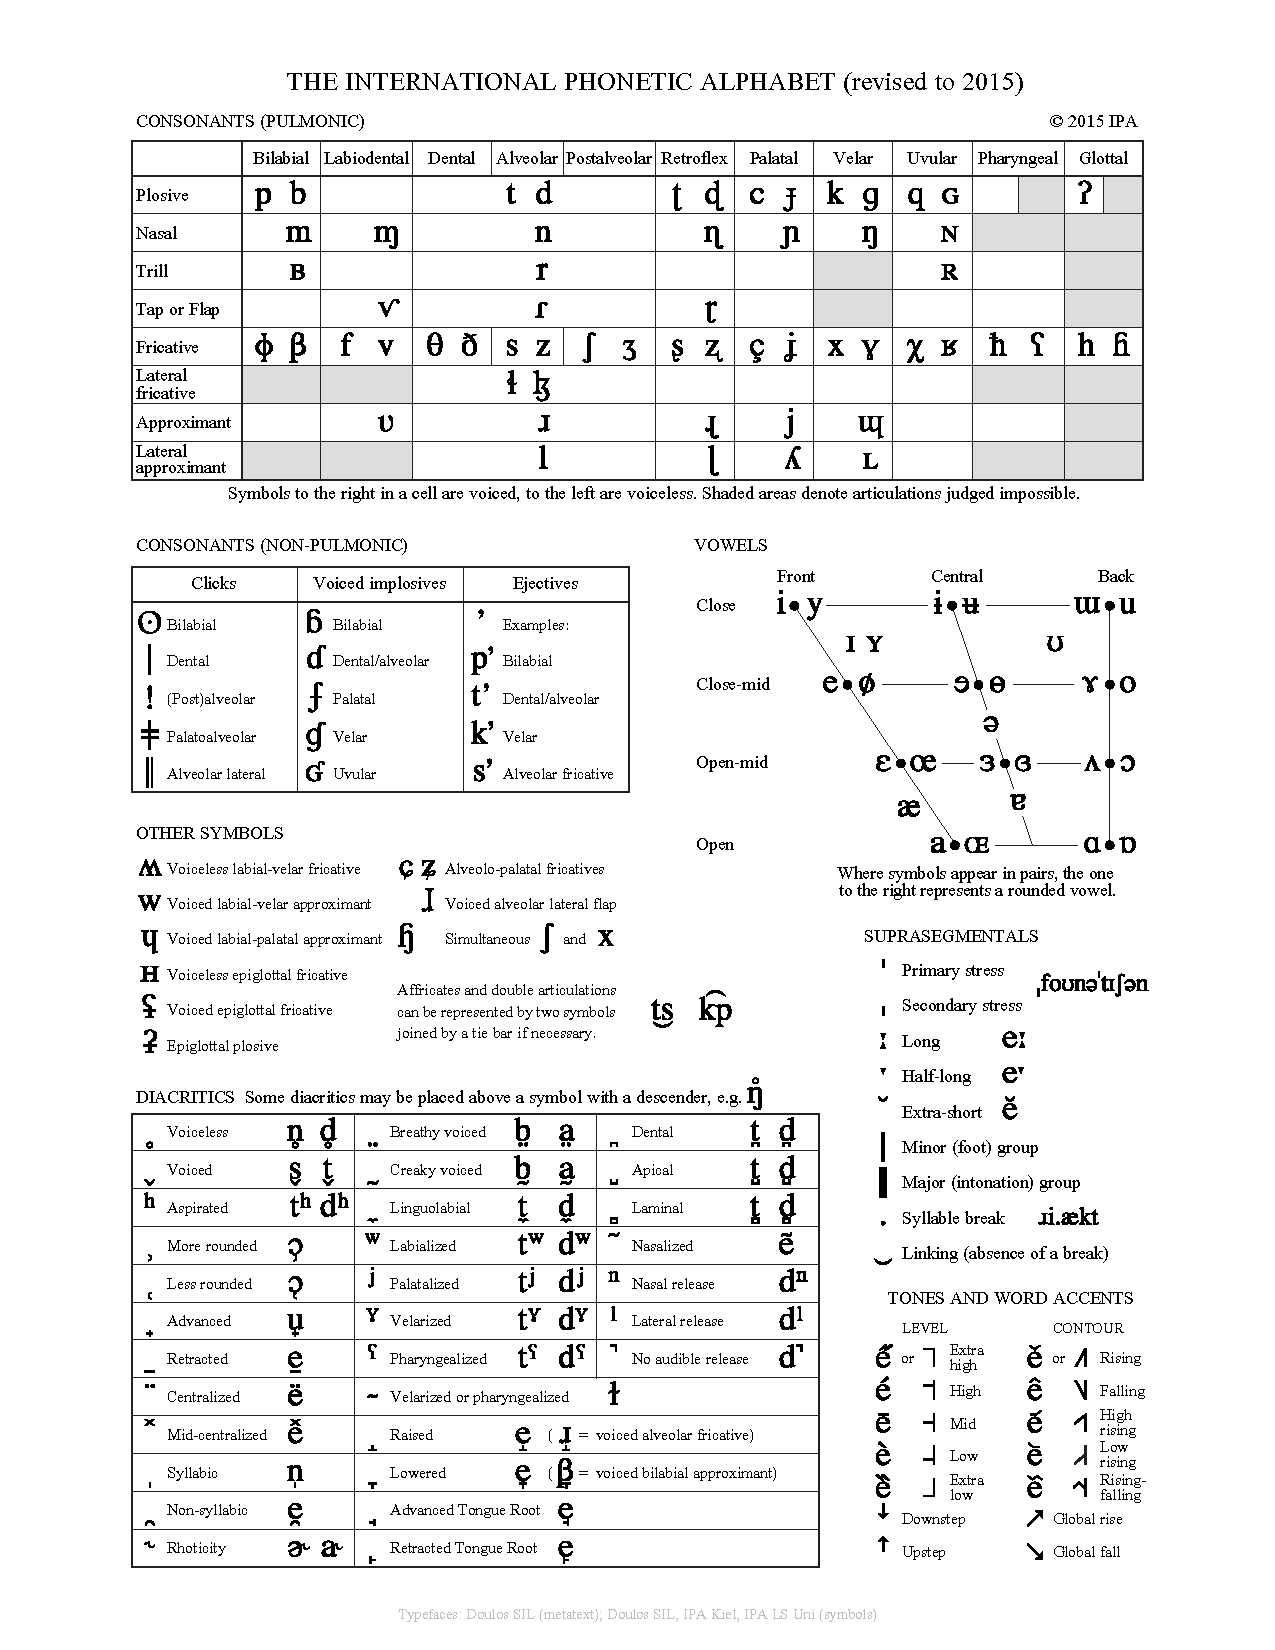
\includegraphics[width=1.3\linewidth]{ipa_chart.pdf}
    \end{center}
    \stepcounter{myfigure}
    \caption[Full IPA chart]{This is the full IPA chart, last updated in 2015}
    \label{fig:ipa_chart}
  \end{figure}

